\documentclass[11pt,t]{beamer}
% xcolor and define colors -------------------------
\usepackage{xcolor}

% https://www.viget.com/articles/color-contrast/
\definecolor{purple}{HTML}{695693}
\definecolor{navy}{HTML}{567293}
\definecolor{ruby}{HTML}{9a2515}
\definecolor{alice}{HTML}{107895}
\definecolor{daisy}{HTML}{EBC944}
\definecolor{coral}{HTML}{F26D21}
\definecolor{kelly}{HTML}{829356}
\definecolor{cranberry}{HTML}{E64173}
\definecolor{jet}{HTML}{131516}
\definecolor{asher}{HTML}{555F61}
\definecolor{slate}{HTML}{314F4F}

% Main theme colors
\definecolor{accent}{HTML}{107895}
\definecolor{accent2}{HTML}{9a2515}

\newcommand\navy[1]{{\color{navy}#1}}
\newcommand\purple[1]{{\color{purple}#1}}
\newcommand\kelly[1]{{\color{kelly}#1}}
\newcommand\ruby[1]{{\color{ruby}#1}}
\newcommand\alice[1]{{\color{alice}#1}}
\newcommand\daisy[1]{{\color{daisy}#1}}
\newcommand\coral[1]{{\color{coral}#1}}
\newcommand\cranberry[1]{{\color{cranberry}#1}}
\newcommand\slate[1]{{\color{slate}#1}}
\newcommand\jet[1]{{\color{jet}#1}}
\newcommand\asher[1]{{\color{asher}#1}}

\newcommand\bgNavy[1]{{\colorbox{navy!80!white}{\textcolor{white}{#1}}}}
\newcommand\bgPurple[1]{{\colorbox{purple!80!white}{\textcolor{white}{#1}}}}
\newcommand\bgKelly[1]{{\colorbox{kelly!80!white}{\textcolor{white}{#1}}}}
\newcommand\bgRuby[1]{{\colorbox{ruby!80!white}{\textcolor{white}{#1}}}}
\newcommand\bgAlice[1]{{\colorbox{alice!80!white}{\textcolor{white}{#1}}}}
\newcommand\bgDaisy[1]{{\colorbox{daisy!80!white}{\textcolor{white}{#1}}}}
\newcommand\bgCoral[1]{{\colorbox{coral!80!white}{\textcolor{white}{#1}}}}
\newcommand\bgCranberry[1]{{\colorbox{cranberry!80!white}{\textcolor{white}{#1}}}}


% Beamer Options -------------------------------------

% Background
\setbeamercolor{background canvas}{bg = white}

% Change text margins
\setbeamersize{text margin left = 15pt, text margin right = 15pt} 

% \alert
\setbeamercolor{alerted text}{fg = accent2}

% Frame title
\setbeamercolor{frametitle}{bg = white, fg = jet}
\setbeamercolor{framesubtitle}{bg = white, fg = accent}
\setbeamerfont{framesubtitle}{size = \small, shape = \itshape}

% Block
\setbeamercolor{block title}{fg = white, bg = accent2}
\setbeamercolor{block body}{fg = jet, bg = jet!10!white}

% Title page
\setbeamercolor{title}{fg = jet}
\setbeamercolor{subtitle}{fg = accent}

%% Custom \maketitle and \titlepage
\setbeamertemplate{title page}
{
    %\begin{centering}
        \vspace{20mm}
        {\Large \usebeamerfont{title}\usebeamercolor[fg]{title}\inserttitle}\\ \vskip0.25em%
        \ifx\insertsubtitle\@empty%
        \else%
          {\usebeamerfont{subtitle}\usebeamercolor[fg]{subtitle}\insertsubtitle\par}%
        \fi% 
        {\vspace{10mm}\insertauthor}\\
        {\color{asher}\small{\insertdate}}\\
    %\end{centering}
}

% Table of Contents
\setbeamercolor{section in toc}{fg = accent!70!jet}
\setbeamercolor{subsection in toc}{fg = jet}

% Button 
\setbeamercolor{button}{bg = accent}

% Remove navigation symbols
\setbeamertemplate{navigation symbols}{}

% Optional: page numbers at bottom
\addtobeamertemplate{navigation symbols}{}{%
    \usebeamerfont{footline}%
    \hspace{1em}%
    \alice{\insertframenumber/\inserttotalframenumber}
    \vspace*{1.5mm}
}


% Table and Figure captions
\setbeamercolor{caption}{fg=jet!70!white}
\setbeamercolor{caption name}{fg=jet}
\setbeamerfont{caption name}{shape = \itshape}

% Bullet points

%% Fix left-margins
\settowidth{\leftmargini}{\usebeamertemplate{itemize item}}
\addtolength{\leftmargini}{\labelsep}

%% enumerate item color
\setbeamercolor{enumerate item}{fg = accent}
\setbeamerfont{enumerate item}{size = \small}
\setbeamertemplate{enumerate item}{\insertenumlabel.}

%% enumerate subitem color
\setbeamercolor{enumerate subitem}{fg = accent!60!white}
\setbeamerfont{enumerate subitem}{size = \small}
\setbeamertemplate{enumerate subitem}{\insertenumlabel.}

%% itemize
\setbeamercolor{itemize item}{fg = accent!70!white}
\setbeamerfont{itemize item}{size = \small}
\setbeamertemplate{itemize item}[circle]

%% right arrow for subitems
\setbeamercolor{itemize subitem}{fg = accent!60!white}
\setbeamerfont{itemize subitem}{size = \small}
\setbeamertemplate{itemize subitem}{$\rightarrow$}

\setbeamertemplate{itemize subsubitem}[square]
\setbeamercolor{itemize subsubitem}{fg = jet}
\setbeamerfont{itemize subsubitem}{size = \small}

% References

%% Bibliography Font, roughly matching aea
\setbeamerfont{bibliography item}{size = \footnotesize}
\setbeamerfont{bibliography entry author}{size = \footnotesize, series = \bfseries}
\setbeamerfont{bibliography entry title}{size = \footnotesize}
\setbeamerfont{bibliography entry location}{size = \footnotesize, shape = \itshape}
\setbeamerfont{bibliography entry note}{size = \footnotesize}

\setbeamercolor{bibliography item}{fg = jet}
\setbeamercolor{bibliography entry author}{fg = accent!60!jet}
\setbeamercolor{bibliography entry title}{fg = jet}
\setbeamercolor{bibliography entry location}{fg = jet}
\setbeamercolor{bibliography entry note}{fg = jet}

%% Remove bibliography symbol in slides
\setbeamertemplate{bibliography item}{}





% Links ----------------------------------------------

\usepackage{hyperref}
\hypersetup{
  colorlinks = true,
  linkcolor = accent2,
  filecolor = accent2,
  urlcolor = accent2,
  citecolor = accent2,
}


% Line spacing --------------------------------------
\usepackage{setspace}
% \setdisplayskipstretch{2}
\setstretch{1.3}


% \begin{columns} -----------------------------------
\usepackage{multicol}


% Fonts ---------------------------------------------
% Beamer Option to use custom fonts
\usefonttheme{professionalfonts}

% \usepackage[utopia, smallerops, varg]{newtxmath}
% \usepackage{utopia}
\usepackage[sfdefault,light]{roboto}

% Small adjustments to text kerning
\usepackage{microtype}



% Remove annoying over-full box warnings -----------
\vfuzz2pt 
\hfuzz2pt


% Table of Contents with Sections
\setbeamerfont{myTOC}{series=\bfseries, size=\Large}
\AtBeginSection[]{
        \frame{
            \frametitle{Roadmap}
            \tableofcontents[current]   
        }
    }


% References ----------------------------------------
\usepackage[
    citestyle= authoryear,
    style = authoryear,
    natbib = true, 
    backend = biber
]{biblatex}

% Smaller font-size for references
\renewcommand*{\bibfont}{\small}

% Remove "In:"
\renewbibmacro{in:}{}

% Color citations for slides
\newenvironment{citecolor}
    {\footnotesize\begin{color}{accent2}}
    {\end{color}}

\newcommand{\citetcolor}[1]{{\footnotesize\textcolor{gray}{\citet{#1}}}}
\newcommand{\citepcolor}[1]{{\footnotesize\textcolor{gray}{\citep{#1}}}}

% Tables -------------------------------------------
% Tables too big
% \begin{adjustbox}{width = 1.2\textwidth, center}
\usepackage{adjustbox}
\usepackage{array}
\usepackage{threeparttable, booktabs, adjustbox}
    
% Fix \input with tables
% \input fails when \\ is at end of external .tex file

\makeatletter
\let\input\@@input
\makeatother

% Tables too narrow
% \begin{tabularx}{\linewidth}{cols}
% col-types: X - center, L - left, R -right
% Relative scale: >{\hsize=.8\hsize}X/L/R
\usepackage{tabularx}
\newcolumntype{L}{>{\raggedright\arraybackslash}X}
\newcolumntype{R}{>{\raggedleft\arraybackslash}X}
\newcolumntype{C}{>{\centering\arraybackslash}X}

% Figures

% \imageframe{img_name} -----------------------------
% from https://github.com/mattjetwell/cousteau
\newcommand{\imageframe}[1]{%
    \begin{frame}[plain]
        \begin{tikzpicture}[remember picture, overlay]
            \node[at = (current page.center), xshift = 0cm] (cover) {%
                \includegraphics[keepaspectratio, width=\paperwidth, height=\paperheight]{#1}
            };
        \end{tikzpicture}
    \end{frame}%
}

% subfigures
\usepackage{subfigure}

% Strikeout text
\usepackage{cancel}

% Highlight slide -----------------------------------
% \begin{transitionframe} Text \end{transitionframe}
% from paulgp's beamer tips
\newenvironment{transitionframe}{
    \setbeamercolor{background canvas}{bg=accent!60!black}
    \begin{frame}\color{accent!10!white}\LARGE\centering
}{
    \end{frame}
}


% Table Highlighting --------------------------------
% Create top-left and bottom-right markets in tabular cells with a unique matching id and these commands will outline those cells
\usepackage[beamer,customcolors]{hf-tikz}
\usetikzlibrary{calc,fit,shapes.misc,backgrounds}
\usepackage{pgfplots}
\pgfplotsset{compat = newest}
\usetikzlibrary{positioning, arrows.meta}
\usepgfplotslibrary{fillbetween}

% halo around text
%https://tex.stackexchange.com/questions/18472/tikz-halo-around-text
\usepackage[outline]{contour} 
\contourlength{1.2pt}
\tikzset{
  contour text/.style={node contents={\contour{white}{#1}}},
  halo text node/.style={circle, draw, pattern=north east lines}
}


\def\arraystretch{0.75}

% To set the hypothesis highlighting boxes red.
\newcommand\marktopleft[1]{%
    \tikz[overlay,remember picture] 
        \node (marker-#1-a) at (0,1.5ex) {};%
}
\newcommand\markbottomright[1]{%
    \tikz[overlay,remember picture] 
        \node (marker-#1-b) at (0,0) {};%
    \tikz[accent!80!jet, ultra thick, overlay, remember picture, inner sep=4pt]
        \node[draw, rectangle, fit=(marker-#1-a.center) (marker-#1-b.center)] {};%
}


\author{Michael Karas}
\title{Lecture 11 - Monopoly and Market Power}
\subtitle{ECON 3070 - Intermediate Microeconomic Theory}
\date{March XX, 2025}


\begin{document}

\begin{frame}
  \titlepage
\end{frame}

\begin{frame}{Overview}
  Up until now, we have assumed that there are a large number of producers and consumers in the market

  \begin{itemize}
    \item Producers are assumed to have very little market power
    
    \item They are unable to individually impact the market price (price takers)
     
    \item A result of this assumption is that total welfare is maximized
  \end{itemize}
\end{frame}

\begin{frame}{Overview}
  In this chapter, we will look at the other extreme.

  \begin{itemize}
    \item A market where only one firm produces the good
    \item And that firm controls the market
    \item They have complete market power
    \item And as we will see, they set the market price so as to maximize their own profit
  \end{itemize}
\end{frame}

\begin{frame}{Monopoly Examples}
  DeBeers 
  \begin{itemize}
    \item Controlled 80\% of the diamond market by 2000.
  \end{itemize}

  \bigskip
  Microsoft Windows (in 1990s)
  \begin{itemize}
    \item Accounted for over 90\% of the market for operating systems.
  \end{itemize}

  \bigskip
  Google
  \begin{itemize}
    \item Ruled to be a monopoly in France, providing about 90\% of web searches in France.
  \end{itemize}
\end{frame}

\begin{frame}{Profit Maximization}
  A perfectly competitive firm maximizes profit by setting 
  
  $$
    MR(Q) = P = MC(Q)
  $$

  \begin{itemize}
    \item That is, a firm will continue producing until the revenue generated by an additional unit of the good is equal to the additional cost of producing it.
    \pause 
    \item A monopolist will follow the same logic, except for the fact that $P$ is not constant
  \end{itemize}
\end{frame}

\begin{frame}{Profit Maximization}
  For a monopoly, price has to go down as you sell more units (because of market demand):

  \begin{figure}
    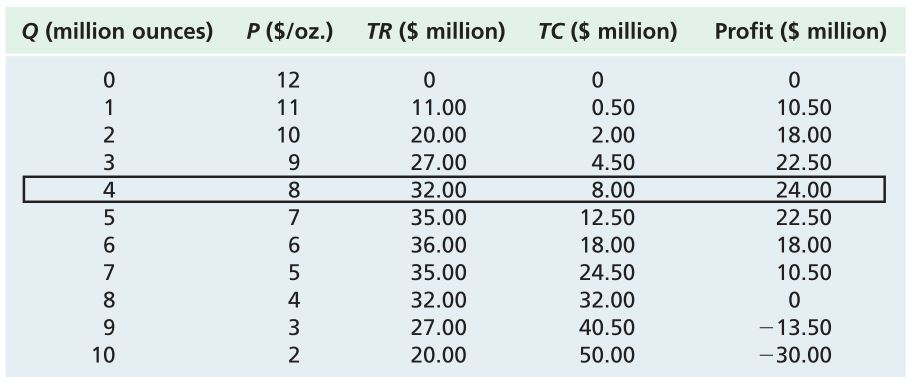
\includegraphics[width=280px]{figures/table11_1.jpg}
  \end{figure}
\end{frame}

\begin{frame}{Profit Maximization}
  As the monopolist produces more, they push the price down.

  \begin{itemize}
    \item For a while, producing more leads to higher revenue (while MR is positive)
    
    \item But after a while, raising the price pushes away too many customers (when MR becomes negative)
  \end{itemize}

  \bigskip
  Meanwhile, total cost is constantly increasing
\end{frame}

\begin{frame}{Profit Maximization}
  The firm will keep increasing output until the additional revenue generated by the last unit is equal to the additional cost incurred in it's production.

  \bigskip
  That is, until $MR(Q) = MC(Q)$

  \bigskip\pause
  This is the \textbf{profit-maximization condition for a monopolist}.
\end{frame}

\begin{frame}{Profit Maximization}
  \begin{columns}[T]
    \vspace{0pt}
    \begin{column}{.55\textwidth}
      \begin{figure}
        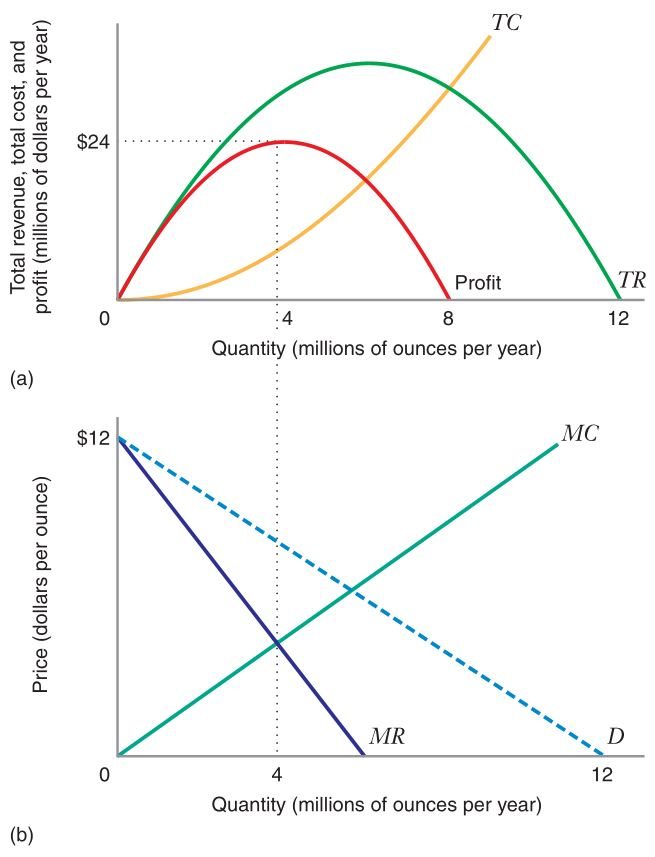
\includegraphics[width=0.8\textwidth]{figures/fig11_2.jpg}
      \end{figure}
  
      \vspace*{50mm} % Ensures columns are up top; delete if you want columns centered on page
    \end{column}
    
    \hfill
    
    \begin{column}{.45\textwidth}
      {\color{accent}\rule{\linewidth}{2pt}}
  
      \begin{itemize}
        \item Total Revenue is no longer linear (since you have to lower price to sell more units)
        
        \item The maximizing profit is when $MR(Q) = MC(Q)$
      \end{itemize}
    \end{column}
  \end{columns}
\end{frame}

\begin{frame}{\bgCranberry{Try It Yourself}}
  If the monopolist is producing where marginal revenue exceeds marginal cost, then the monopolist should $\rule{2cm}{0.15mm}$ to maximize profits.

  \begin{enumerate}[A)]
    \item produce more
    \item produce less
    \item stop producing
    \item raise the price
  \end{enumerate}
\end{frame}

\begin{frame}{Marginal Revenue Review}
  For a perfectly competitive firm, \textit{marginal revenue equals the market price}

  \begin{itemize}
    \item If a P.C. firm sells an additional unit, the price does not change, so $MR(Q) = P$
  \end{itemize}

  \bigskip
  For a monopolist, the relationship does not hold

  \begin{itemize}
    \item In order to sell more units, the monopolist must lower the price on all units
    
    \item Their revenue increases by the market price $P$, but falls by a small amount for every unit they were previously selling.
  \end{itemize}
\end{frame}

\begin{frame}{Marginal Revenue}
  \begin{columns}[T]
    \vspace{0pt}
    \begin{column}{.55\textwidth}
      \begin{figure}
        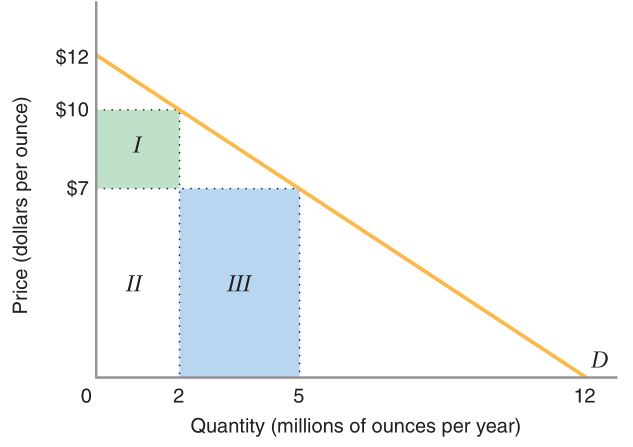
\includegraphics[width=\textwidth]{figures/fig11_3.jpg}
      \end{figure}
  
      \vspace*{50mm} % Ensures columns are up top; delete if you want columns centered on page
    \end{column}
    
    \hfill
    
    \begin{column}{.45\textwidth}
      {\color{accent}\rule{\linewidth}{2pt}}
  
      \textbf{Original Revenue:} I + II

      \textbf{New Revenue:} II + III

      \bigskip
      \begin{itemize}
        \item Revenue grows because you sell 3 more units (+ III)
        \item Revenue shrinks because you sell the original 2 units for a lower price (- I)
      \end{itemize}
    \end{column}
  \end{columns}
\end{frame}

\begin{frame}{Marginal Revenue}
  In the graph, area $III$ represents the revenue gained from selling additional units by lowering the price

  \begin{itemize}
    \item This is called the \textbf{quantity effect}
  \end{itemize}

  \bigskip
  Area $I$ represents revenue lost on the \textbf{inframarginal units}, or the units that were previously sold at the higher price.

  \begin{itemize}
    \item This is called the \textbf{price effect}
  \end{itemize}
\end{frame}

\begin{frame}{Marginal Revenue}
  The price and quantity effects move marginal revenue in opposite directions:

  \begin{itemize}
    \item Quantity effect (area $III$) = Price $\times$ change in quantity = $P \Delta Q$
    
    \item Price effect (area $I$) = Quantity $\times$ change in price = $Q \Delta P$
  \end{itemize}


  \bigskip\pause
  The change in total revenue is given by:
  $$
    \Delta TR = \text{Price effect} + \text{Quantity Effect} = P\Delta Q + Q\Delta P
  $$
\end{frame}

\begin{frame}{Marginal Revenue}
  If we divide this change in total revenue by the change in quantity, we get the marginal revenue:
  $$
    MR = \frac{\Delta TR}{\Delta Q} = \frac{P\Delta Q + Q\Delta P}{\Delta Q}=P+Q\frac{\Delta P}{\Delta Q}
  $$
  
  \bigskip
  The first part corresponds to the quantity effect
  \begin{itemize}
    \item Another unit is sold at price P
  \end{itemize}
  
  \bigskip
  The second part is the price effect.
  \begin{itemize}
    \item The price of $Q$ previous units falls by $\frac{\Delta P}{\Delta Q}$
  \end{itemize}
\end{frame}

\begin{frame}{Monopolist's Profit Maximization Problem}
  Let's show that the monopolist's profit maximizing optimality condition holds, using the tools we've seen so far.

  \bigskip
  Because a monopolist's output impacts the price, price is no longer constant, but instead a function of Q. The monopolist's problem becomes
  $$
    \max_Q \pi= P(Q) Q - TC(Q),
  $$
  where now $P$ depends on $Q$
\end{frame}

\begin{frame}{Monopolist's Profit Maximization Problem}
  To find the profit maximizing quantity, take the derivative w.r.t $Q$, and set equal to zero
  $$
    \frac{d\pi}{dQ} = \underbrace{Q \frac{dP(Q)}{dQ} + P(Q)}_{MR(Q)} - \underbrace{\frac{dTC(Q)}{dQ}}_{MC(Q)} = 0
  $$

  \bigskip
  Rearranging:
  $$
    MR(Q^*)=MC(Q^*)
  $$
\end{frame}

\begin{frame}{Monopolist's Profit Maximization Problem}
  Example: Suppose that a monopolist faces the market demand curve $P(Q) = 40 - Q$, and total cost function $TC(Q) = Q^2$.

  \bigskip
  Remember that the monopolist's optimality condition is $MR(Q) = MC(Q)$. Let's find MR and MC.
  \begin{align*}
    MR(Q) &= \frac{dTR(Q)}{dQ}      \\
          &= \frac{d}{dQ}((40 - Q) * Q) \\
          &= \frac{d}{dQ}(40Q - Q^2)  \\
          &= 40 - 2Q
  \end{align*}
\end{frame}

\begin{frame}{Monopolist's Profit Maximization Problem}
  Calculating marginal cost:
  $$
    MC(Q) = \frac{\partial TC(Q)}{\partial Q} = 2Q
  $$ 

  \bigskip\pause
  From our optimality condition, $MR(Q) = MC(Q)$:
  $$
    40 - 2Q = 2Q \implies Q^* = 10
  $$

  \bigskip\pause
  Finally, the market price will be the price at which the firm sells exactly $Q^*$ units:
  $$
    P(10) = 40-10=30
  $$
\end{frame}

\begin{frame}{\bgCranberry{Try It Yourself}}
  Suppose that market demand in a given market can be written as $P(Q) = 20 - \frac{1}{3} Q^2$. What is the marginal revenue function for a monopolist in this market?
  \pause The firm faces a marginal cost function given by $MC(Q) = 4Q^2$, find the monopolist's profit-maximizing quantity of output.
\end{frame}

\begin{frame}{Monopolist's Profit Maximization Problem}
  \begin{figure}
    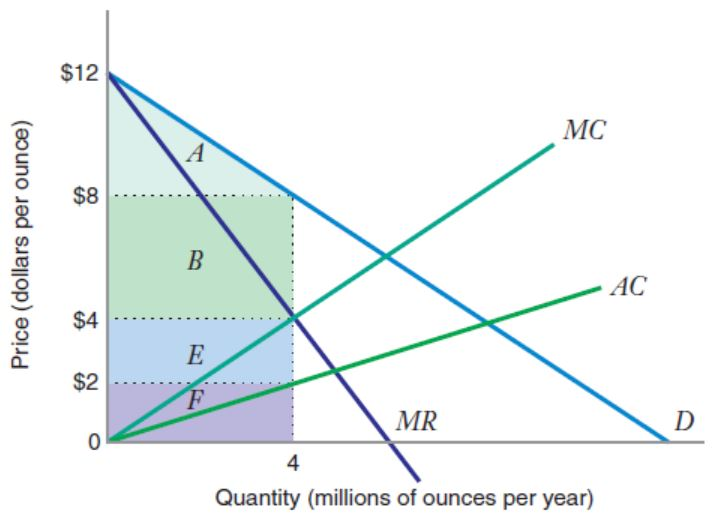
\includegraphics[width=250px]{figures/fig11_5.jpg}
  \end{figure}
\end{frame}

\begin{frame}{Implications}
  Three important points about the equilibrium:

  \bigskip
  \begin{enumerate}
    \item The profit-maximizing price exceeds marginal cost of the last unit supplied.

    \item Economic profits are not zero in the long run. \textbf{(why?)}

    \item Consumers still receive some consumer surplus.
  \end{enumerate}
\end{frame}

\begin{frame}{\bgCranberry{Try It Yourself}}
  For a monopolist,
  \begin{enumerate}[A)]
    \item selling price is greater than marginal revenue.
    \item selling price is equal to marginal revenue.
    \item selling price is less than marginal revenue.
    \item selling price may be above or below marginal revenue; it depends on the price buyers are willing to pay.
  \end{enumerate}
\end{frame}

\begin{frame}{Price Elasticity of Demand and the Profit-Maximizing Price}
  The gap between the price that a firm charges, and their marginal cost, will depend on how sensitive consumers are to a change in price.

  \begin{itemize}
    \item If consumers are very price sensitive, the monopolist will set the price relatively low (the price effect dominates)

    \item If the opposite is true, the monopolist will set the price higher (the quantity effect dominates)
  \end{itemize}

  \bigskip\pause
  Intuitively, if a firm faces more competition from an outside industry, consumers will be more price-sensitive and the monopolist's price will be lower.
\end{frame}

\begin{frame}{Price Elasticity of Demand and the Profit-Maximizing Price}
  \begin{figure}
    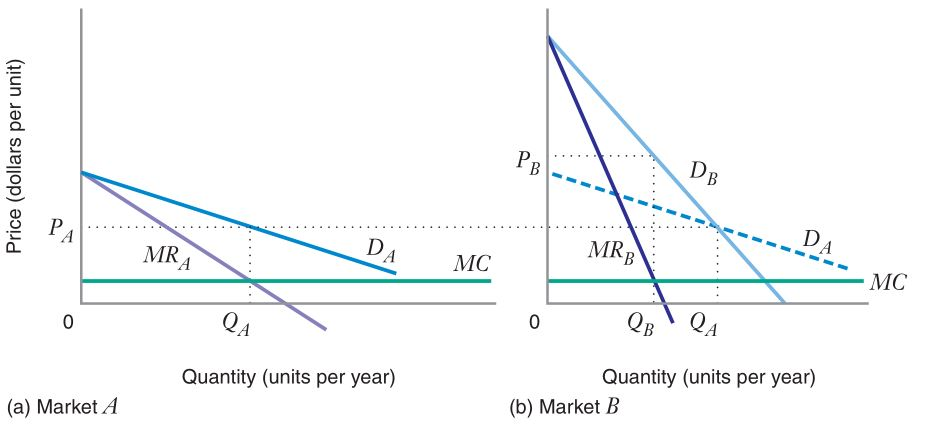
\includegraphics[width=280px]{figures/fig11_7.jpg}
  \end{figure}
\end{frame}

\begin{frame}{Marginal Revenue and Price Elasticity of Demand}
  Formally, we can use the equation for marginal revenue to express the relationship between MR and price:
  \begin{align*}
    MR &= P + Q \frac{\Delta P}{\Delta Q}                         \\
       &= P + Q \frac{\Delta P}{\Delta Q} * \frac{P}{P}           \\
       &= P + P \frac{\Delta P}{\Delta Q} * \frac{Q}{P}           \\
       &= P \Big(1 + \frac{\Delta P}{\Delta Q} * \frac{Q}{P} \Big)
  \end{align*}
\end{frame}

\begin{frame}{Marginal Revenue and Price Elasticity of Demand}
  Remember that price elasiticy of demand is given by

  \begin{equation}
    \epsilon_{Q,P}=\frac{\Delta Q}{Q} /\frac{\Delta P}{P}\text{ or } \frac{\Delta Q}{\Delta P}*\frac{P}{Q}
  \end{equation}

  \bigskip
  Therefore, marginal revenue can be expressed as
  $$
    MR=P\Big(1+\frac{1}{\epsilon_{Q,P}}\Big)
  $$
\end{frame}

\begin{frame}{Marginal Revenue and Price Elasticity of Demand}
  \begin{figure}
    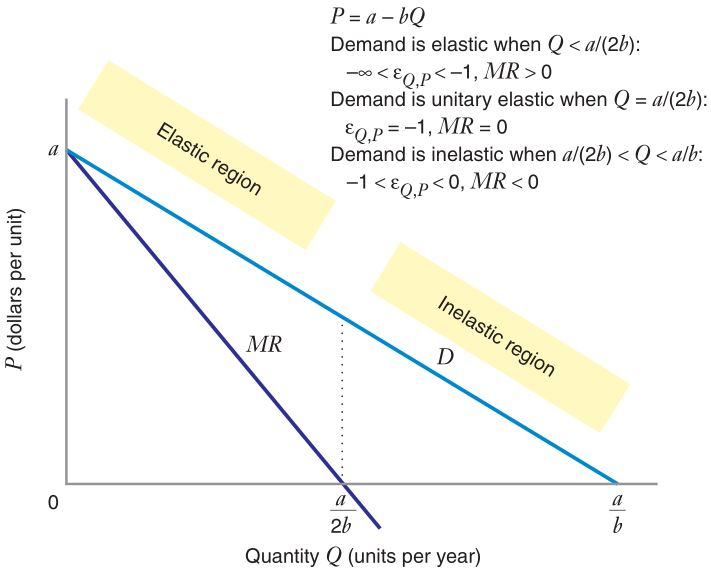
\includegraphics[width=240px]{figures/fig11_8.jpg}
  \end{figure}
\end{frame}

\begin{frame}{Marginal Cost and Price Elasticity of Demand}
  Remember that, at $Q^*$, $MR(Q^*)=MC(Q^*)$.

  \bigskip
  We can therefore rewrite the previous equation as
  $$
    MC(Q^*)= P \Big( 1 + \frac{1}{\epsilon_{Q,P}} \Big)
  $$

  \pause\bigskip
  Rearranging: 
  $$
  P = MC(Q^*) \frac{1}{1 + \frac{1}{\epsilon_{Q,P}}}
  $$
  Since $(1 + \frac{1}{\epsilon_{Q,P}}) < 1$, you will charge a price above your cost
\end{frame}

% \begin{frame}{Inverse Elasticity Pricing Rule}
%   If we rewrite this equation, we get the \textbf{inverse elasticity pricing rule}:
%   $$
%     \frac{P^*-MC^*}{P^*}=-\frac{1}{\epsilon_{Q,P}}
%   $$
%   This gives a relationship between a firm's optimal markup and the price elasticity of demand.
% \end{frame}

\begin{frame}{Differentiated Products}
  Monopolists aren't the only firms that face a downward-sloping demand curve.

  \begin{itemize}
    \item Many firms sell products that are unique (so they do not operate in a perfectly competitive market), but they still face competitors
  \end{itemize}

  \bigskip
  Think of breakfast cereals (Lucky Charms, Frosted Flakes, Cap'n Crunch).

  \begin{itemize}
    \item These firms still charge a price above their marginal cost
  \end{itemize}
\end{frame}

\begin{frame}{The Lerner Index}
  If a monopolist faces fewer competitors (few close substitutes), consumers will be less price sensitive and the firm's markup will be greater.

  \bigskip\pause
  Intuitively, we can use the firm's markup as a measure of market power.

  \begin{itemize}
    \item This is known as the \textbf{Lerner Index}.
    
    \item Firms with greater market power, and thus a higher markup, will score higher on the Lerner Index.
  \end{itemize}

\end{frame}

\begin{frame}{\bgCranberry{Try It Yourself}}
  Inverse demand for a monopolist's product is given by $P(Q) = 300-6Q$ while the monopolist's marginal cost is given by $MC(Q) = 3Q$. 
  
  \only<1>{What is the profit-maximizing quantity of output for this monopolist?}\only<2>{What is the profit-maximizing price for this monopolist?}\only<3>{At the profit-maximizing quantity of output, what is the firm's marginal cost of the final unit produced?}
\end{frame}

% \begin{frame}{Shifts in Market Demand}
%   \bigskip

%   With perfect competition, we assumed that marginal costs were increasing.

%   Otherwise, as a firm produced more, their costs would fall, and they would never stop producing.

%   This assumption can be relaxed somewhat for a monopolist.

%   In either case, however, if demand shifts outward, the monopolist will produce more.
% \end{frame}

% \begin{frame}{Shifts in Market Demand}
%   \bigskip

%   However, whether the prices goes up or down will depend on the shape of the MC curve.

%   If marginal costs are increasing in Q, the firm will charge a higher price.

%   If marginal costs are decreasing in Q, the price may be higher or lower.
% \end{frame}

\begin{frame}{Comparative Statics: Shifts in Market Demand}
  \begin{figure}
    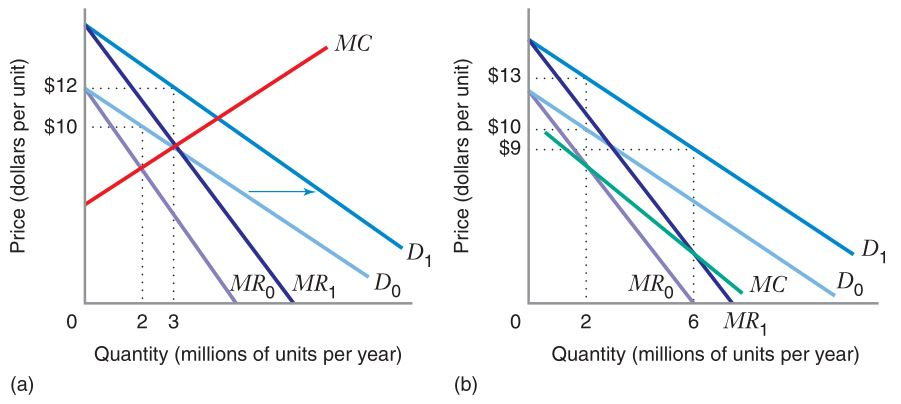
\includegraphics[width=280px]{figures/fig11_10.jpg}
  \end{figure}
\end{frame}

% \begin{frame}{Shifts in Marginal Cost}
%   \bigskip

%   If MC increases, Q always decreases.

%   This is because the marginal revenue curve is downward sloping.

%   Thus, P will always increase (because Q fell).

%   And profit will fall (because Q is smaller, and marginal cost for every unit is higher)
% \end{frame}

\begin{frame}{Comparative Statics: Shifts in Marginal Cost}
  \begin{figure}
    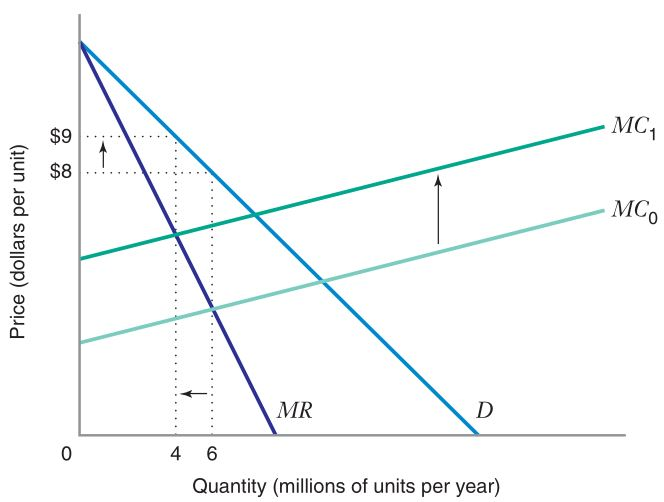
\includegraphics[width=240px]{figures/fig11_12.jpg}
  \end{figure}
\end{frame}

\begin{frame}{Multi-plant Monopoly}
  Let's consider the case where a monopolist has two production plants. Think of a utility company with multiple power plants.

  \begin{itemize}
    \item Each plant has a separate marginal cost; $MC_1$ and $MC_2$.
    
    \item How should the plant allocate production between the two plants?
  \end{itemize}

\end{frame}

\begin{frame}{Multi-plant Monopoly}
  Suppose the firm produces equal amounts at both plants:

  \begin{itemize}
    \item Because the marginal cost is different at each plant, the monopoly can produce fewer units at the higher-cost plant, and more units at the lower cost plant
    
    \item By doing so, marginal cost of the final unit is decreased and profit rises
  \end{itemize}
\end{frame}

\begin{frame}{Multi-plant Monopoly}
  \begin{figure}
    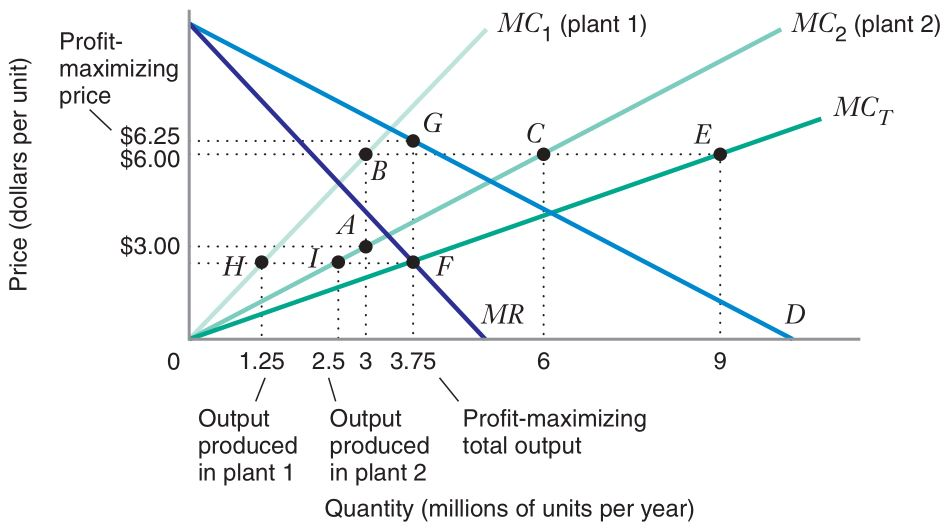
\includegraphics[width=310px]{figures/fig11_14.jpg}
  \end{figure}
\end{frame}

\begin{frame}{Multi-plant Monopoly}
  This exercise illustrates the importance of the \textbf{multi-plant marginal cost curve}
  \begin{itemize}
    \item This curve denotes the marginal cost of producing a given quantity in the lowest-cost way
    
    \item Each additional unit will be produced at the plant where the marginal cost is the lowest
  \end{itemize}

  \bigskip
  So the multi-plant marginal cost curve is found by simply summing the individual MC curves horizontally
\end{frame}

\begin{frame}{Multi-plant Monopoly}
  The production decision is the same a single-plant monopolist by using the multi-plant marginal cost curve

  \begin{itemize}
    \item A multi-plant monopolist can find the profit maximizing quantity by setting marginal revenue equal to the multi-plant marginal cost
    
    \item The market price is the price that will allow the firm to sell all of it's output from both plants
  \end{itemize}
\end{frame}

\begin{frame}{\bgCranberry{Try It Yourself}}
  A monopolist owns two plants in which to produce product A.  The marginal cost of producing A is increasing, but currently is lower in plant 1 than in plant 2.  How should the monopolist allocate production?

  \begin{enumerate}[A)]
    \item Produce all output in plant 1.
    \item Produce all output in plant 2.
    \item Produce 50 percent in plant 1 and 50 percent in plant 2.
    \item Produce in plant 1 up to the point where marginal costs are equated across the plants.
  \end{enumerate}
\end{frame}

% \begin{frame}{Output Choice with Two Markets}
%   Suppose that a monopolist wishes to sell it's output good in two markets.

%   We will assume that they must sell it at the same price in both markets (no price discrimination).

%   Suppose that demand in market 1 is given by $Q_1(P)$ and demand in market 2 is given by $Q_2(P)$.

%   Total revenue depends on the number of units sold in both markets: $Q=Q_1(P) +Q_2(P)$.

%   Total cost depends on $Q$ as well.
% \end{frame}

% \begin{frame}{Output Choice with Two Markets}
%   \bigskip

%   As we know, overall demand is simply the horizontal sum of two individual (or in this case, market) demand curves.

%   The optimal quantity for the monopolist is then given by $MC(Q)=MR(Q)$.
% \end{frame}

\begin{frame}{Profit Maximization by a Cartel}
  A \textbf{cartel} is a group of producers that determine the price and output in a market through \textbf{collusion}

  \begin{itemize}
    \item An example is the Organization of Petroleum Exporting Countries (OPEC)
    \item This was a group of some of the world's largest oil producers, including Kuwait, Saudi Arabia, Iran and Venezuela
  \end{itemize}

  \bigskip
  When a cartel works as intended, it acts as a monopoly firm with multiple plants
\end{frame}

\begin{frame}{Profit Maximization by a Cartel}
  At the profit-maximizing solution, the cartel allocates production between the two firms such that marginal cost is equal.

  \bigskip
  For example, suppose that two firms collude.

  Then for $Q^* = Q^*_1 + Q^*_2$, the following should be true:
  $$
    MR(Q^*) = MC_1(Q_1^*) \text{ and } MR(Q^*) = MC_2(Q^*_2)
  $$
\end{frame}

\begin{frame}{Profit Maximization by a Cartel}
  \begin{figure}
    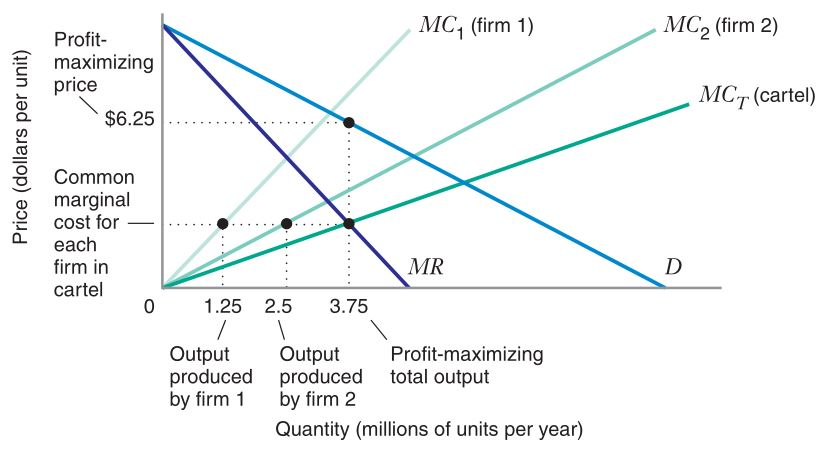
\includegraphics[width=280px]{figures/fig11_15.jpg}
  \end{figure}
\end{frame}

\begin{frame}{Profit Maximization by a Cartel}
  So if cartels are so great for producers, why aren't there more of them?
  \bigskip\pause

  \begin{itemize}
    \item They are illegal (we will see why in a few slides).
    
    \item They are hard to keep together (one firm can lower the price and sell more units).
  \end{itemize}
\end{frame}

\begin{frame}{The Welfare Economics of Monopoly}
  Suppose a perfectly competitive industry was monopolized
  \begin{itemize}
    \item For example, one company bought all of its competitors
  \end{itemize}

  Then the industry supply curve would become that firm's marginal cost curve...

  \begin{itemize}
    \item And that firm would set output such that $MC(Q^*) = MR(Q^*)$
    
    \item Quantity produced would fall, and price would rise
  \end{itemize}
\end{frame}

\begin{frame}{The Welfare Economics of Monopoly}
  \begin{figure}
    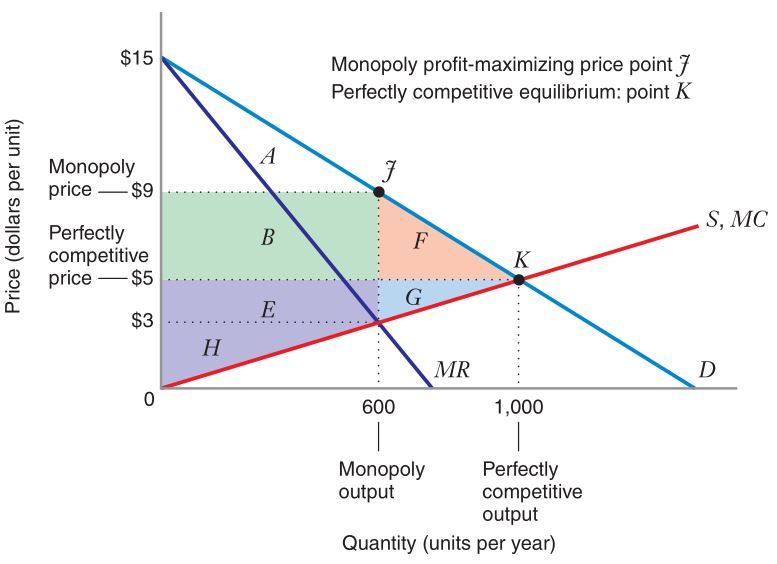
\includegraphics[width=260px]{figures/fig11_16a.jpg}
  \end{figure}
\end{frame}

\begin{frame}{The Welfare Economics of Monopoly}
  G and F are the \textbf{deadweight loss due to monopoly}
  \begin{itemize}
    \item The monopolist's surplus increases by area B (but they lose G)
    
    \item Consumer surplus decreases by B and F
  \end{itemize}

  \bigskip
  By raising the price and lowering output, the firm has eliminated transactions that are welfare increasing.

  \begin{itemize}
    \item That is, transactions where the marginal benefit to consumers is greater than the marginal cost to the producer
  \end{itemize}
\end{frame}

\begin{frame}{The Welfare Economics of Monopoly}
  This additional producer surplus encourages firms to acquire monopoly power

  \begin{itemize}
    \item Activities aimed at creating or preserving monopoly power are called \textbf{rent-seeking activities}
  \end{itemize}

  \bigskip\pause
  For example, lobbying the government to regulate an industry in order to prevent entry (think of Uber in London)

  \begin{itemize}
    \item A firm would be willing to spend some of that additional surplus on rent-seeking activities in order to maintain its market power (through lobbying)
  \end{itemize}
\end{frame}

\begin{frame}{The Welfare Economics of Monopoly}
  This is why the government typically fights to keep firms from gaining too much market power.
  \begin{itemize}
    \item With some exceptions, the U.S government does not allow monopolies to exist (Microsoft, for example)
    
    \item Cartels are also illegal in the U.S.
  \end{itemize}

  \bigskip Enforcement of this varies over time though ...
\end{frame}

\begin{frame}{Why do Monopoly Markets Exist?}
  One reason may be that the total cost incurred by a single firm to produce output for the market might be lower than the combined total cost for two or more firms
  
  \bigskip 
  An example is satellite television:
  \begin{itemize}
    \item Large up-front fixed costs (building a satellite and shooting it into space).
    \item One firm needs one satellite to serve the whole market.
    \item Two firms need two satellites.
  \end{itemize}

  \bigskip
  This is known as a \textbf{natural monopoly}.
\end{frame}

\begin{frame}{Why do Monopoly Markets Exist?}
  Another example is an electric company.

  \begin{itemize}
    \item Again, large up-front fixed costs (building transmission lines throughout a city)
    \item Would be very expensive for two firms to compete for customers in one city
  \end{itemize}

  \bigskip
  Economies of scale imply it's cheaper for one firm to produce instead of two firms
\end{frame}

\begin{frame}{Why do Monopoly Markets Exist?}
  A natural monopoly is an example of a \textbf{barrier to entry}.
  
  \begin{itemize}
    \item Barriers to entry allow an incumbent to earn a profit, while making entry unprofitable for newcomers
    \item Without barriers to entry, if an incumbent is earning a profit, more firms will enter
    \item Profit will go to zero
  \end{itemize}
\end{frame}

\begin{frame}{Why do Monopoly Markets Exist?}
  Examples

  \begin{itemize}
    \item Large fixed costs 
    \item Social media platforms (Snapchat, Facebook, Instagram) have positive network externalities
    \item Government regulation (taxis)
  \end{itemize}
\end{frame}

\begin{frame}{Why do Monopoly Markets Exist?}
  \textbf{Legal barriers to entry} exist when an incumbent firm is legally protected against competitors.

  \bigskip
  Patents are the biggest example:

  \begin{itemize}
    \item Drug companies are given monopoly power by the government in order to recoup their R\&D costs
    \item Once the patent expires, new entrants come to the market, and the price usually falls.
  \end{itemize}
\end{frame}

\begin{frame}{Why do Monopoly Markets Exist?}
  \textbf{Strategic barriers to entry} result when an incumbent firm takes explicit steps to deter entry.

  \bigskip
  An example is starting a price war if a new firm enters.
\end{frame}

\begin{frame}{\bgCranberry{Try It Yourself}}
  Economists consider monopolists:

  \begin{enumerate}[A)]
    \item to be efficient, since they earn greater profits than perfect competitors.
    \item to be inefficient since all consumer surplus is transferred to the monopolist in the form of profits.
    \item to be inefficient since they earn less producers' surplus than all firms taken together in a competitive market.
    \item to be inefficient since the monopolist restricts output from the competitive level, thus creating dead-weight loss.
  \end{enumerate}
\end{frame}

\end{document}
